\documentclass[conference]{IEEEtran}
\IEEEoverridecommandlockouts
\usepackage{cite}
\usepackage{amsmath,amssymb}
\usepackage{graphicx}
\usepackage{booktabs}
\usepackage{multirow}
\usepackage[table]{xcolor}
\usepackage{siunitx}
\usepackage{tikz}
\usetikzlibrary{positioning,arrows.meta,fit,backgrounds,calc}
\usepackage{balance}
\usepackage{url}
\usepackage[hidelinks]{hyperref}
\sisetup{detect-all, group-minimum-digits=5, quantity-product={~}}

\begin{document}
\bstctlcite{IEEEexample:BSTcontrol}

\title{What Waiting Buys: Live Soccer Game State\\Reconstruction from Broadcast Video}

\author{\IEEEauthorblockN{Saurav Rijal}
\IEEEauthorblockA{\textit{Department of Computer Science}\\
\textit{Texas State University}\\
San Marcos, TX, USA}}

\maketitle

\begin{abstract}
Game state reconstruction converts a single moving broadcast feed into a top-down minimap that gives each player's pitch position, identity, team, role, and jersey number. Published systems run offline: they cluster teams over the whole clip, read jersey numbers anywhere in a track and propagate them backward, and merge tracklets afterward, and they report accuracy without processing speed. We build a pipeline in which every decision is causal and evaluate it as a live system, varying the one parameter such a system controls: the output delay, that is, how far ahead it may look before committing an output. The pipeline combines a role-aware detector, a tracker whose camera-motion compensation is shared with keyframe pitch calibration, online team clustering, and confidence-gated jersey voting. On the 49 labeled SoccerNet test clips it reaches 34.6 points of the official game-state accuracy metric with no lookahead and 43.6 with the whole clip, and 1~s of delay adds 2.5 points (95\% confidence interval 2.1 to 2.9). Its perception stages sustain 32 frames per second on one graphics processing unit (GPU) alongside the jersey reader. On the validation split, with all other attributes taken from ground truth, going from live output to the whole clip improves jersey recognition by 17.3 points and team assignment by 9.1. Error budgets and oracle experiments locate the remaining gap in attribute errors and in detection and association errors, chiefly identities that break into several tracks; a fine-tuned jersey reader with higher crop accuracy did not improve test results.
\end{abstract}

\begin{IEEEkeywords}
Camera calibration, game state reconstruction, multi-object tracking, real-time systems, sports analytics
\end{IEEEkeywords}

\section{Introduction}
Professional soccer tracking relies on calibrated multi-camera installations in stadiums. Broadcast-only tracking is offered commercially, but its methods are unpublished, and lower leagues, academies, and many women's competitions have only broadcast or single-camera video. The SoccerNet game state reconstruction (GSR) task~\cite{somers2024gsr} made the broadcast-to-minimap problem measurable. Its metric, GS-HOTA, credits a predicted player only when its pitch position and all of its attributes (role, team, and jersey number) are correct.

The strongest GSR systems are built for an offline leaderboard~\cite{golovkin2025minimap,soccernet2025results,oo2026broadcast2pitch}. The 2024 challenge winner runs its raw tracking stage in real time, but its team clustering and tracklet split-and-merge are post-processing steps over the whole clip, and it reports accuracy for that setting only~\cite{golovkin2025minimap}. A live product cannot see the whole clip. It can, however, hold its output back by a bounded amount, as broadcast graphics already do; in estimation theory this is fixed-lag smoothing~\cite{sarkka2013bayesian}. This paper asks how much GSR accuracy each second of output delay buys, and in which component.

Our contributions are:
\begin{enumerate}
\item A GSR pipeline in which every decision is causal, combining a role-aware detector, a tracker with camera-motion compensation, keyframe calibration with optical-flow propagation, online team clustering, and delayed-commit jersey voting, evaluated with the official GS-HOTA implementation.
\item GS-HOTA as a function of output delay, end to end and per component, on the SoccerNet-GSR validation and test splits, with clip-level bootstrap confidence intervals and paired tests.
\item A measured real-time operating point of 32 frames per second (FPS) for the perception stages on one GPU with the jersey reader running concurrently, together with a per-stage latency budget.
\item An error budget, oracle analysis, and negative results that locate the remaining accuracy gap.
\end{enumerate}

\section{Related Work}
\textbf{Game state reconstruction.} Somers \emph{et al.}~\cite{somers2024gsr} introduced the SoccerNet-GSR dataset, the GS-HOTA metric, and an offline baseline that runs at about 1.1~FPS. The 2024 winner~\cite{golovkin2025minimap} combines a YOLOv5 detector, learned camera calibration, and DeepSORT~\cite{wojke2017deepsort} in pitch coordinates; its tracking stage runs at up to 80~FPS with TensorRT, but team clustering and tracklet post-processing operate over the whole clip. Entries in the 2025 challenge~\cite{soccernet2025results} use vision-language models for jersey and role recognition, whole-clip tracklet merging, or both, and report no speed. Broadcast2Pitch~\cite{oo2026broadcast2pitch} adds keypoint-and-line calibration with vision-language tracklet refinement and notes that its language model is costly for real-time use; it reports no runtime.

\textbf{Tracking.} Our tracker belongs to the ByteTrack family~\cite{zhang2022bytetrack}, which associates low-confidence detections in a second pass, and uses camera-motion compensation as in BoT-SORT~\cite{aharon2022botsort} and McByte~\cite{stanczyk2025mcbyte}. Sports-specific trackers such as Deep-EIoU~\cite{huang2024deepeiou} add expanded box overlap and appearance features. Accuracy is measured with higher order tracking accuracy (HOTA)~\cite{luiten2021hota}; sports benchmarks include SportsMOT~\cite{cui2023sportsmot} and SoccerNet-Tracking~\cite{cioppa2022soccernettracking}.

\textbf{Calibration, team, and jersey recognition.} Broadcast pitch calibration methods include TVCalib~\cite{theiner2023tvcalib}, NBJW~\cite{gutierrez2024nbjw}, BroadTrack~\cite{magera2025broadtrack}, and PnLCalib~\cite{gutierrez2024pnlcalib}, which we use. Team assignment is commonly unsupervised clustering of appearance~\cite{koshkina2021contrastive}. Koshkina and Elder~\cite{koshkina2024jersey} recognize jersey numbers with a legibility classifier, pose-guided torso crops, and a PARSeq scene-text recognizer~\cite{bautista2022parseq} fine-tuned on SoccerNet data; we use their released models.

\textbf{Accuracy under delay.} Streaming perception~\cite{li2020streaming} scores detectors by the state of the world when an output becomes available. Near-online tracking~\cite{choi2015nomt} and NOOUGAT~\cite{missaoui2026noougat} trade latency against temporal context for image-space multi-object tracking. To our knowledge, no prior work reports GSR accuracy as a function of output delay, where the attributes that dominate the metric, not only the tracks, depend on lookahead.

\section{Problem Formulation}
\textbf{Task.} Given broadcast frames $x_1,\dots,x_T$, the system outputs for each frame $t$ a set of tracked people, each with a pitch position in meters, a track identity, a role (player, goalkeeper, or referee), a team (left or right, by the side of the pitch the team defends), and a jersey number.

\textbf{Output delay.} A system with delay $L$ computes its output for frame $t$ from frames $x_1,\dots,x_{t+L}$. $L=0$ is fully live, and $L=\infty$, the whole clip, is the offline setting. At 25~FPS, $L=25$, $125$, and $250$ frames correspond to 1, 5, and 10~s. The wall-clock delay of a deployed system is $L$ plus its processing latency (Section~\ref{sec:speed}).

\textbf{Metric.} HOTA~\cite{luiten2021hota} at localization threshold $\alpha$ is $\mathrm{HOTA}_\alpha=\sqrt{\mathrm{DetA}_\alpha\cdot\mathrm{AssA}_\alpha}$, the geometric mean of detection accuracy (DetA) and association accuracy (AssA), averaged over $\alpha\in\{0.05,0.10,\dots,0.95\}$. GS-HOTA~\cite{somers2024gsr} replaces image intersection-over-union with a Gaussian similarity of pitch distance (5~m tolerance) and counts a match only if role, team, and jersey number also agree. GS-DetA and GS-AssA denote its detection and association components. We also report \emph{pitch HOTA}, the same matching without attributes, which isolates localization and tracking. All HOTA-family scores are given on a 0--100 scale except in Section~\ref{sec:nothelp}, where image-space tracking HOTA is on a 0--1 scale.

\section{Method}
Fig.~\ref{fig:pipeline} shows the pipeline. Neural stages run on the GPU, and geometry, tracking, and decisions run on the CPU, in overlapping threads.

\begin{figure*}[t]
\centering
\resizebox{\textwidth}{!}{%
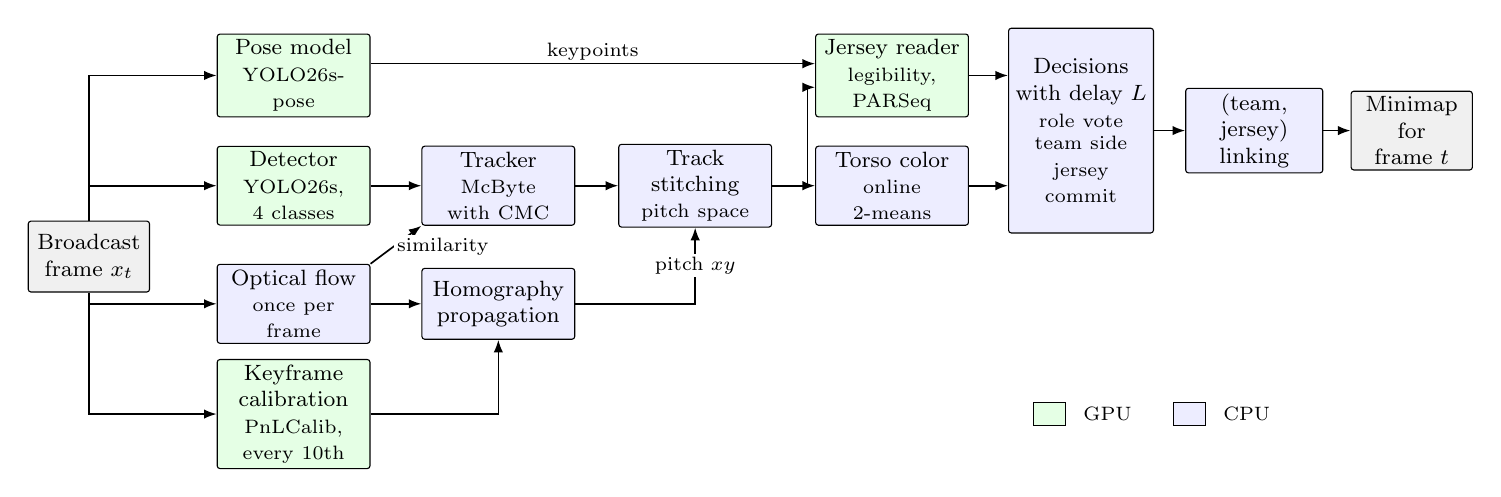
\begin{tikzpicture}[font=\footnotesize, x=1cm, y=1cm,
  box/.style={draw, rounded corners=1pt, minimum height=9mm, text width=18mm, align=center, inner sep=2pt},
  gpu/.style={box, fill=green!10}, cpu/.style={box, fill=blue!7}, io/.style={box, fill=gray!12, text width=14mm},
  lab/.style={font=\scriptsize, fill=white, inner sep=1pt},
  arr/.style={-{Latex[length=1.6mm]}, semithick}]
\node[io]  (frame) at (0,1.0)     {Broadcast\\frame $x_t$};
\node[gpu] (pose)  at (2.6,3.3)   {Pose model\\{\scriptsize YOLO26s-pose}};
\node[gpu] (det)   at (2.6,1.9)   {Detector\\{\scriptsize YOLO26s, 4 classes}};
\node[cpu] (flow)  at (2.6,0.4)   {Optical flow\\{\scriptsize once per frame}};
\node[gpu] (kf)    at (2.6,-1.0)  {Keyframe calibration\\{\scriptsize PnLCalib, every 10th}};
\node[cpu] (trk)   at (5.2,1.9)   {Tracker\\{\scriptsize McByte with CMC}};
\node[cpu] (prop)  at (5.2,0.4)   {Homography\\propagation};
\node[cpu] (rep)   at (7.7,1.9)   {Track stitching\\{\scriptsize pitch space}};
\node[gpu] (jer)   at (10.2,3.3)  {Jersey reader\\{\scriptsize legibility, PARSeq}};
\node[cpu] (team)  at (10.2,1.9)  {Torso color\\{\scriptsize online 2-means}};
\node[cpu, minimum height=26mm, text width=17mm] (dec) at (12.6,2.6) {Decisions with delay $L$\\[2pt]{\scriptsize role vote\\team side\\jersey commit}};
\node[cpu, text width=16mm] (lnk) at (14.8,2.6) {(team, jersey) linking};
\node[io]  (map)   at (16.8,2.6) {Minimap for frame $t$};
\draw[arr] (frame.north) |- (pose.west);
\draw[arr] (frame.north) |- (det.west);
\draw[arr] (frame.south) |- (flow.west);
\draw[arr] (frame.south) |- (kf.west);
\draw[arr] (det) -- (trk);
\draw[arr] (flow.north east) -- node[lab, right, pos=0.45]{similarity} (trk.south west);
\draw[arr] (flow) -- (prop);
\draw[arr] (kf.east) -| (prop.south);
\draw[arr] (trk) -- (rep);
\draw[arr] (prop.east) -| node[lab, pos=0.75]{pitch $xy$} (rep.south);
\draw[arr] ([yshift=1.5mm]pose.east) -- node[lab, above, pos=0.5]{keypoints} ([yshift=1.5mm]jer.west);
\draw[arr] (rep) -- (team);
\draw[arr] (rep.east) -- ++(0.45,0) |- ([yshift=-1.5mm]jer.west);
\draw[arr] (jer.east) -- (jer.east -| dec.west);
\draw[arr] (team.east) -- (team.east -| dec.west);
\draw[arr] (dec) -- (lnk);
\draw[arr] (lnk) -- (map);
\node[draw, fill=green!10, minimum width=4mm, minimum height=3mm, inner sep=0] (lg1) at (12.2,-1.0) {};
\node[right=1mm of lg1, font=\scriptsize] (t1) {GPU};
\node[draw, fill=blue!7, minimum width=4mm, minimum height=3mm, inner sep=0, right=4mm of t1] (lg2) {};
\node[right=1mm of lg2, font=\scriptsize] {CPU};
\end{tikzpicture}}
\caption{Live GSR pipeline. One optical-flow estimate per frame, masked with the previous frame's tracked boxes, serves both camera-motion compensation (CMC) in the tracker and propagation of the image-to-pitch homography between keyframe calibrations, which run asynchronously in the live runner and synchronously in accuracy experiments. All decisions use only evidence up to frame $t+L$.}
\label{fig:pipeline}
\end{figure*}

\subsection{Detection and pose}
A YOLO26s detector~\cite{ultralytics} initialized from weights pretrained on COCO~\cite{lin2014coco} is fine-tuned on the SoccerNet-GSR training split with four classes (player, goalkeeper, referee, ball), so that roles come from the detector. We train on every fifth frame of 52 training clips at $1280$-pixel input with batch size 16, the Ultralytics default optimizer, learning-rate schedule, and augmentation, and seed 0, holding out 5 training clips for early stopping (patience 10, at most 40 epochs; training stopped after 29). On the held-out clips it reaches 0.852 mean average precision at 0.5 intersection-over-union (mAP@0.5). Detections above confidence 0.1 are passed to the tracker. A YOLO26s-pose model runs on the same full frame and supplies body keypoints for jersey crops.

\subsection{Shared camera motion}
For each frame we detect up to 400 Shi--Tomasi corners~\cite{shi1994good} on a grayscale image downscaled to 640~pixels wide, masking the boxes tracked in the previous frame, and track them with pyramidal Lucas--Kanade flow~\cite{lucas1981iterative,bouguet2001pyramidal} ($21\times21$ window, four pyramid levels) into the current frame. From the same correspondences we fit, with random sample consensus (RANSAC)~\cite{fischler1981ransac} at a 1.5-pixel threshold, a homography $M_t$ mapping frame $t$ to frame $t-1$, used for calibration, and a four-degree-of-freedom similarity, used as the tracker's camera-motion compensation (CMC). A frame with fewer than 40 inliers is treated as a camera cut.

\subsection{Tracking and identity repair}
We use McByte~\cite{stanczyk2025mcbyte} as implemented in the open-source \texttt{trackers} library~\cite{roboflowtrackers} with its default parameters and its mask stage disabled, replacing its built-in motion estimator with the shared similarity. Broken tracks are repaired online in pitch space: when a new track appears, it is linked to a recently lost track of the same role group if the gap $g$ is at most 150 frames, the pitch distance is at most $2+0.4g$~m (about 10~m/s), and the normalized distance between the new track's torso color feature and the lost track's running average (exponential smoothing factor 0.9) is below 3.

\subsection{Keyframe calibration with propagation}
PnLCalib~\cite{gutierrez2024pnlcalib}, with its released SoccerNet-trained weights and $960\times540$ input, estimates the camera on every tenth frame. Between keyframes, the image-to-pitch homography is carried forward with the frame-to-frame motion~\cite{hartley2003multiple},
\begin{equation}
H_t = H_\kappa \prod_{j=\kappa+1}^{t} M_j ,
\end{equation}
where $\kappa$ is the latest keyframe. A player's pitch position is the image of the bottom-center of its box under $H_t$. For accuracy evaluation, keyframe calibrations are applied synchronously, and a detected cut immediately triggers a new calibration. The live runner (Section~\ref{sec:speed}) runs the calibrator asynchronously, brings each late result up to the current frame by chaining the stored motions, and after a cut waits for the next scheduled keyframe.

\subsection{Role and team}
A track's role is the majority detector class over the last 25 frames and the available lookahead. For team assignment, each player box yields a color feature: the mean and standard deviation in CIELAB space of the non-grass pixels (hue 30--90 and saturation above 60 in OpenCV's HSV scale) in the torso region, which spans 15--55\% of the box height and the central half of its width. After standardizing the features, a two-cluster $k$-means model is re-fitted every 25 frames on all features seen up to $t+L$ (at most 4000 samples), warm-started from the previous centroids to keep labels stable. No team is output until 25 frames of evidence exist. Each track is assigned by its mean feature, and the cluster whose players have the lower mean pitch $x$ is labeled ``left.'' Goalkeepers take the side of the half they stand in.

\subsection{Jersey numbers with delayed commit}
For each player box at least 40~pixels tall, the torso crop spans the shoulder and hip keypoints of the pose detection that overlaps the box with intersection-over-union of at least 0.5, with a 5-pixel margin, when at least three of the four keypoints, including a shoulder, have confidence of 0.3 or more; otherwise it spans 10--55\% of the box height. The legibility classifier and PARSeq reader of~\cite{koshkina2024jersey} give, for crop $i$ observed at frame $t_i$, a legibility probability $\ell_i$ and a distribution $p_i(n)$ over numbers $n\in\{0,\dots,99\}$. Track $q$ accumulates the gated evidence
\begin{multline}
s_q(n)=\sum_{i\in q,\ t_i\le t+L} \mathbf{1}\!\left[\ell_i\ge0.3 \wedge \max_m p_i(m)\ge\rho\right]\\
\cdot\,\ell_i\,p_i(n),
\end{multline}
where $\mathbf{1}[\cdot]$ is the indicator function, and commits $\hat n=\arg\max_n s_q(n)$ once $s_q(\hat n)\ge\tau$ and $s_q(\hat n)\ge r\sum_n s_q(n)$, with $\rho=0.97$, $\tau=4$, and $r=0.6$ chosen on the validation split. Before committing, the track reports no number. Once a track commits a (team, jersey) pair owned by an identity that is not visible in the current frame, it takes over that identity.

\section{Experimental Setup}
\textbf{Data.} SoccerNet-GSR~\cite{somers2024gsr} provides 30-s clips at 25~FPS and $1920\times1080$ resolution with public labels for 57 training, 58 validation, and 49 test clips; labels of the 36 challenge clips are hidden. All design choices were made on the validation split, and each configuration was evaluated once on the test split with frozen settings.

\textbf{Evaluation.} We use the official SoccerNet implementation of GS-HOTA. Confidence intervals come from 2000 bootstrap resamples of clips (seed 0)~\cite{efron1993bootstrap}; each resample is recombined with the evaluator's own pooling, so it is an exact GS-HOTA. Paired comparisons resample the same clips for both systems.

\textbf{Implementation.} Experiments ran on an NVIDIA H100 NVL GPU with an Intel Xeon Gold 6548Y+ CPU, using PyTorch 2.6 (CUDA 12.4), Ultralytics 8.4.174, \texttt{trackers} 2.6.1, OpenCV 4.14, and TensorRT 10.13~\cite{tensorrt}. Accuracy was measured with PyTorch 32-bit floating-point (FP32) models; the live runner uses TensorRT 16-bit floating-point (FP16) engines for the detector and pose model, whose accuracy we report in Section~\ref{sec:speed}. The jersey models run in a separate process because their dependencies require an older PyTorch.

\section{Results}

\subsection{Error budget}
Table~\ref{tab:budget} degrades perfect ground truth one factor at a time on the validation split. Because GS-HOTA requires every attribute to match, team side and jersey numbers dominate: swapping the two team labels costs as much as omitting team entirely. Calibration must be accurate well below 1~m, whereas role confusion and missed detections are comparatively cheap.

\begin{table}[t]
\caption{Error Budget: Ground Truth with One Factor Degraded (Validation)}
\label{tab:budget}
\centering
\footnotesize
\begin{tabular}{@{}lr@{}}
\toprule
Degradation & GS-HOTA \\
\midrule
None & 100.0 \\
Team sides swapped / no team & 22.1 / 21.5 \\
No jersey numbers & 36.7 \\
Pitch noise 0.5 / 1 / 2 m & 94.3 / 75.5 / 39.3 \\
Per-frame calibration offset 1 / 2 m & 75.6 / 39.4 \\
Track IDs broken every 10 / 2 s & 63.4 / 30.5 \\
Referees and goalkeepers labeled player & 88.2 \\
10\% of detections missed & 90.0 \\
\bottomrule
\end{tabular}
\end{table}

\subsection{Which components benefit from waiting}
Fig.~\ref{fig:components} scores one component at a time, taking every other attribute from ground truth. Jersey numbers are legible only intermittently, so evidence keeps arriving for many seconds and the curve rises up to the whole clip (+17.3 points). Team color settles within about 10~s (+9.1); a variant that fits the clusters once, after 1~s of evidence or on the whole clip offline, and votes per box scores higher with the whole clip (95.5 versus 92.3) but lower at every finite delay, so we use online re-fitting throughout. Calibration is causal by construction and was not evaluated with lookahead smoothing; its line in Fig.~\ref{fig:components} is constant. Keyframe calibration on every tenth frame with propagation keeps 99\% of per-frame accuracy (82.0 versus 82.5 calibration-only GS-HOTA; 0.58~m versus 0.53~m median error) while calling the calibrator on 9.8\% of frames, and without fresh keyframes propagation drifts to a 4.9~m median error.

\begin{figure}[t]
\centering
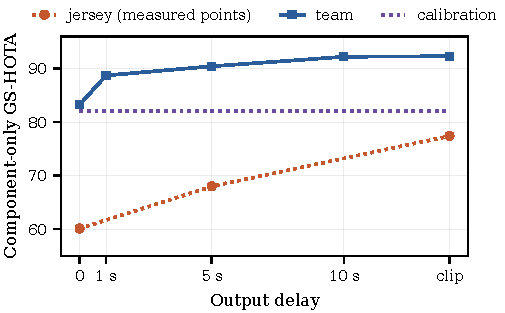
\includegraphics[width=\columnwidth]{figures/components.pdf}
\caption{Component-only GS-HOTA versus output delay on the validation split, with all other attributes from ground truth. Jersey recognition was evaluated at 0~s, 5~s, and the whole clip; calibration does not use lookahead and is shown as a constant.}
\label{fig:components}
\end{figure}

\subsection{End-to-end accuracy versus output delay}
Table~\ref{tab:main} and Fig.~\ref{fig:delay} report end-to-end results. On the test split, accuracy rises from 34.6 GS-HOTA with no delay to 43.6 with the whole clip. Absolute confidence intervals are wide (about $\pm$3 to $\pm$4 points) because clips differ in difficulty, but paired differences are tight: relative to live output, delay adds 2.51 [2.13, 2.93] at 1~s, 5.31 [3.95, 6.82] at 5~s, and 9.04 [5.55, 12.36] with the whole clip, and none of the 2000 resamples shows a gain of zero or less. Because the whole-clip setting is this causal system given more evidence rather than an offline-optimized system, it is a weak upper bound: 1~s recovers 28\% of the gap to it, and 10~s recovers 84\%. GS-AssA rises steadily with delay while GS-DetA dips slightly with the whole clip, likely because whole-clip decisions apply each committed attribute to all of a track's boxes, which propagates wrong commits backward. Pitch HOTA is nearly identical on both splits (66.1 and 66.0), so the higher test score comes from the attributes. Three test clips (identifiers SNGS-126, -131, and -197) are reported to have incorrect team labels~\cite{oo2026broadcast2pitch}; without them, GS-HOTA is 35.6 live and 45.2 with the whole clip.

\begin{table}[t]
\caption{End-to-End Results versus Output Delay}
\label{tab:main}
\centering
\footnotesize
\setlength{\tabcolsep}{3pt}
\begin{tabular}{@{}lccccc@{}}
\toprule
Metric & 0 s & 1 s & 5 s & 10 s & Clip \\
\midrule
\multicolumn{6}{@{}l}{\emph{Test (49 clips)}} \\
GS-HOTA & \textbf{34.6} & \textbf{37.1} & \textbf{39.9} & \textbf{42.1} & \textbf{43.6} \\
\quad 95\% CI & {\scriptsize 31.3--37.8} & {\scriptsize 33.7--40.6} & {\scriptsize 36.0--43.8} & {\scriptsize 38.0--46.3} & {\scriptsize 39.3--47.8} \\
GS-DetA & 24.7 & 26.8 & 28.8 & 30.3 & 29.1 \\
GS-AssA & 48.4 & 51.4 & 55.3 & 58.6 & 65.5 \\
\midrule
\multicolumn{6}{@{}l}{\emph{Validation (58 clips)}} \\
GS-HOTA & 29.5 & 31.6 & 34.3 & 35.9 & 37.9 \\
\bottomrule
\end{tabular}\\[2pt]
\parbox{\columnwidth}{\scriptsize Test intervals are 95\% clip-bootstrap confidence intervals.}
\end{table}

\begin{figure}[t]
\centering
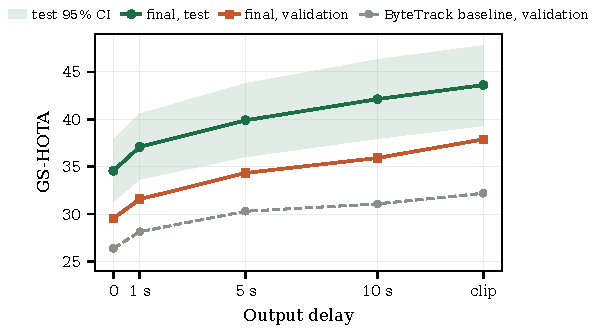
\includegraphics[width=\columnwidth]{figures/delay_curve.pdf}
\caption{End-to-end GS-HOTA versus output delay. The band is the 95\% clip-bootstrap confidence interval on the test split; ``clip'' denotes access to the whole clip.}
\label{fig:delay}
\end{figure}

Table~\ref{tab:compare} places these results next to published test-split numbers. Our live system scores above the official offline baseline, but well below the offline state of the art, whose margin comes from steps unavailable to a causal system: whole-clip tracklet split-and-merge, appearance re-identification across the clip, and vision-language jersey reading.

\begin{table}[t]
\caption{Comparison on the SoccerNet-GSR Test Split}
\label{tab:compare}
\centering
\footnotesize
\setlength{\tabcolsep}{2.4pt}
\begin{tabular}{@{}llcccc@{}}
\toprule
Method & Causal & GS-HOTA & DetA & AssA & Speed \\
\midrule
Baseline~\cite{somers2024gsr} & no & 22.3 & 10.7 & 46.5 & 1.1 FPS \\
Golovkin \emph{et al.}~\cite{golovkin2025minimap}$^\dagger$ & no & 55.8 & 41.7 & 74.9 & -- \\
Broadcast2Pitch~\cite{oo2026broadcast2pitch} & no & 61.5 & 48.5 & 78.0 & -- \\
\midrule
Ours, 0 s delay & yes & 34.6 & 24.7 & 48.4 & 32 FPS$^\ddagger$ \\
Ours, whole clip & no$^\ast$ & 43.6 & 29.1 & 65.5 & -- \\
\bottomrule
\end{tabular}\\[2pt]
\parbox{\columnwidth}{\scriptsize $^\dagger$Test-split values as reported in~\cite{oo2026broadcast2pitch}, which also reports the baseline's DetA and AssA. Baseline speed on an A100 GPU~\cite{somers2024gsr}; the tracking stage of~\cite{golovkin2025minimap} alone runs at up to 80~FPS. $^\ddagger$Perception stages with the jersey reader running concurrently (Section~\ref{sec:speed}). $^\ast$Our causal decision rules given the whole clip.}
\end{table}

Table~\ref{tab:ablation} builds the system up on the validation split. Jersey evidence gating and pose-guided crops give the largest significant gains; stitching helps the live setting; camera-motion compensation and identity linking are within noise end to end.

\begin{table}[t]
\caption{Cumulative Ablation on the Validation Split (GS-HOTA)}
\label{tab:ablation}
\centering
\footnotesize
\setlength{\tabcolsep}{2.2pt}
\begin{tabular}{@{}lcccc@{}}
\toprule
Configuration & Live & Clip & Gain, live & Gain, clip \\
\midrule
ByteTrack, raw jersey reads & 26.4 & 32.2 & -- & -- \\
+ shared CMC (McByte) & 26.5 & 32.0 & {\scriptsize 0.09 [$-$0.44, 0.64]} & {\scriptsize $-$0.23 [$-$1.39, 0.80]} \\
+ jersey evidence gating & 27.8 & 35.2 & {\scriptsize 1.35 [0.80, 1.95]} & {\scriptsize 3.27 [2.26, 4.38]} \\
+ pitch-space stitching & 28.7 & 36.2 & {\scriptsize 0.87 [0.18, 1.61]} & {\scriptsize 0.94 [$-$0.84, 2.66]} \\
+ (team, jersey) linking & 28.7 & 36.4 & {\scriptsize 0.00 [$-$0.18, 0.15]} & {\scriptsize 0.19 [0.02, 0.36]} \\
+ pose-guided crops & \textbf{29.5} & \textbf{37.9} & {\scriptsize 0.87 [0.49, 1.31]} & {\scriptsize 1.51 [0.86, 2.19]} \\
\bottomrule
\end{tabular}\\[2pt]
\parbox{\columnwidth}{\scriptsize Gains are paired clip-bootstrap differences with 95\% confidence intervals, computed before rounding.}
\end{table}

Fig.~\ref{fig:qual} shows one test frame with a 5-s delay. Most players are localized within a few meters and labeled with the correct number, but several are assigned to the wrong team, the dominant error type identified in Table~\ref{tab:budget}.

\begin{figure*}[t]
\centering
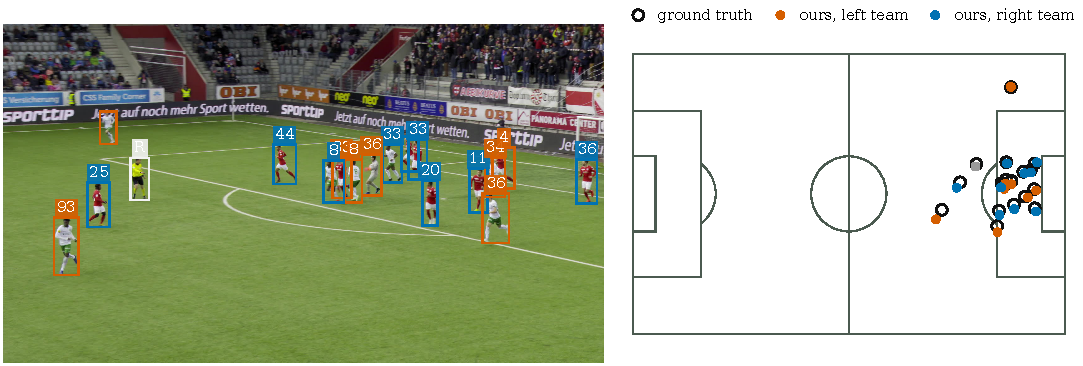
\includegraphics[width=\textwidth]{figures/qualitative.pdf}
\caption{Qualitative result on test clip SNGS-116 (frame 301) with a 5-s delay. Left: boxes colored by predicted team (white: referee) with committed jersey numbers. Right: predicted pitch positions (filled) and ground truth (open). Several players are assigned to the wrong team.}
\label{fig:qual}
\end{figure*}

\subsection{Where the remaining points are}
Table~\ref{tab:oracle} replaces one attribute of live predictions with the ground truth of the matched box. It uses the ByteTrack baseline configuration (26.4 live on validation). Jersey numbers are the largest single lever (+12.7). With these tracks, perfect attributes and positions still cap GS-HOTA at 72; the remaining loss comes from detection and association errors, chiefly fragmentation. In the baseline, each ground-truth identity is split into 2.81 predicted tracks on average, and 74.6\% of the breaks are frame-to-frame identity changes while the player stays visible. The final system reduces this to 2.16 tracks per identity (53.2\% frame-to-frame breaks).

\begin{table}[t]
\caption{Oracle Swaps on End-to-End Predictions of the ByteTrack Baseline (Validation, GS-HOTA)}
\label{tab:oracle}
\centering
\footnotesize
\begin{tabular}{@{}lcc@{}}
\toprule
Ground truth substituted for & Live & Clip \\
\midrule
Nothing (prediction) & 26.4 & 32.2 \\
Role & 27.9 & 33.6 \\
Team & 30.8 & 35.0 \\
Jersey number & 39.0 & 44.1 \\
Team and jersey number & 50.2 & 50.2 \\
All attributes & 60.5 & 60.6 \\
Pitch position & 30.3 & 37.1 \\
Pitch position and all attributes & 72.0 & 72.1 \\
\bottomrule
\end{tabular}
\end{table}

\subsection{Speed}\label{sec:speed}
Table~\ref{tab:speed} lists per-stage latency on an idle GPU for one validation clip (SNGS-021), measured over 300 frames after 30 warm-up frames. TensorRT FP16 engines reduce the detector from 6.6~ms to 5.0~ms and the pose model from 7.0~ms to 5.1~ms at $1280$-pixel input; with these engines in the full pipeline, validation GS-HOTA is 29.9 live and 38.5 with the whole clip, compared with 29.5 and 37.9 with FP32 models, so the faster engines do not reduce accuracy. The live runner overlaps GPU and CPU stages in threads, runs the calibrator asynchronously, and processes 750 frames of the same clip, of which the first 50 are discarded. Its perception stages (decode, detector, pose, optical flow, tracker, calibration, and team features) sustain 44.2~FPS alone, with 44~ms median and 58~ms 95th-percentile latency, and 32.0~FPS (56~ms and 64~ms) while the jersey reader runs concurrently on the same GPU. Under that contention the jersey reader itself takes 15.7~ms per frame at the median and 124~ms at the 95th percentile. The decision stage (stitching, role, team, jersey commit, and linking) costs 0.4~ms per frame when replayed on one CPU thread. Tracker timings from the multi-process sweep in Section~\ref{sec:nothelp} were measured under heavy CPU load and are not comparable to Table~\ref{tab:speed}.

\begin{table}[t]
\caption{Per-Stage Median Latency per Frame on One Idle GPU. The Calibrator Runs on Every Tenth Frame; Its Cost Is Shown Amortized}
\label{tab:speed}
\centering
\footnotesize
\begin{tabular}{@{}llr@{}}
\toprule
Stage & Device & ms \\
\midrule
Frame decode & CPU & 5.6 \\
Detector, PyTorch FP32 / TensorRT FP16 & GPU & 6.6 / 5.0 \\
Pose, PyTorch FP32 / TensorRT FP16 & GPU & 7.0 / 5.1 \\
Optical flow and homography propagation & CPU & 6.9 \\
Tracker & CPU & 1.0 \\
Team color features & CPU & 1.5 \\
Keyframe calibrator (47.7~ms per call) & GPU & 4.8 \\
Jersey legibility and reader (about 13 crops) & GPU & 9.4 \\
Decisions (batch replay) & CPU & 0.4 \\
\bottomrule
\end{tabular}
\end{table}

\subsection{What did not help}\label{sec:nothelp}
\textbf{Better image-space tracking.} On the validation split, image-space HOTA (0--1 scale) is 0.584 for ByteTrack and 0.597 for McByte with its own CMC, which reduces identity switches from 3462 to 2014; with the shared CMC it scores 0.596 with 2015 switches. End-to-end GS-HOTA changes by less than one point (Table~\ref{tab:ablation}) because attributes dominate.

\textbf{A fine-tuned jersey reader.} Fine-tuning PARSeq on 71\,812 weakly labeled legible crops from the training split raised exact accuracy on legible crops of five held-out training clips from 81.0\% to 90.6\% (best of six epochs, selected on the same held-out clips). Crops were labeled with their track's jersey number and kept when the legibility classifier gave at least 0.5; we fine-tuned from the SoccerNet checkpoint with AdamW, learning rate $10^{-4}$, batch size 128, a one-cycle schedule, and RandAugment. At its own validation-tuned gate ($\rho=0.9$), the fine-tuned reader raised jersey-only validation GS-HOTA slightly (60.9 live and 78.1 with the whole clip, versus 60.1 and 77.4 for the pretrained reader at $\rho=0.97$) and end-to-end validation GS-HOTA by 0.5 to 0.8, but changed test GS-HOTA by only 0.10 [$-$0.43, 0.75] live and $-$0.59 [$-$1.66, 0.29] with the whole clip. With ground-truth boxes and a common gate of $\rho=0.9$, both readers produce at least one gated read for 97--98\% of numbered identities, and the pretrained reader produces a correct gated read for more of them (91.9\% versus 84.1\%). Missing legibility therefore explains little of the remaining jersey loss; we attribute it to the time before a number is committed, during which boxes carry no number, and to identity breaks that split a player's evidence across tracks, although we did not measure commit latency directly.

\textbf{Other crops and thresholds.} Wider, lower, and whole-box crops all read worse than the torso band, and a small two-digit classifier trained on tracklet-level labels learned kit appearance rather than digits. Across 13 gate settings ($\rho$ from 0.6 to 0.97, $\tau$ from 2 to 16), live jersey-only GS-HOTA varied between 54.2 and 58.4.

\section{Limitations}
Confidence intervals capture clip sampling but not run-to-run variance, because each configuration was trained and run once. Results are on the public test split; we did not submit to the hidden challenge split, and beyond noting that pitch HOTA is equal on both splits, we did not analyze which attributes or clips make test scores exceed validation scores. Our whole-clip setting is a causal system given more evidence, not an offline-optimized system, which leaves a large gap to the offline state of the art (Table~\ref{tab:compare}). Speed was measured on one clip and one GPU type, with the jersey reader as a separate process, and accuracy was measured with synchronous calibration. The PnLCalib and jersey models were pretrained on SoccerNet data, and we did not check for game overlap with the test clips. All learned components were trained on professional men's broadcast footage, so performance on the lower-league and women's competitions that motivate this work is untested.

\section{Ethics and Licensing}
SoccerNet-GSR contains broadcast footage of professional players, who are identifiable by face and jersey number; we use it under the dataset's research terms and release no new footage. The system estimates player positions and identities, which can support performance analysis but could also be misused for surveillance of individuals; deployment should follow the consent and data-protection rules of the competition and jurisdiction. The calibration models (GPL-2.0) and jersey models (non-commercial license) were used for research measurement only, and the detector framework is licensed under AGPL-3.0.

\section{Data and Code Availability}
SoccerNet-GSR is available from the SoccerNet project under its research terms~\cite{somers2024gsr}. Our code, configurations, per-configuration result files, and the scripts that regenerate every table and figure in this paper are available at \url{https://github.com/Rizsaurav/realtime-sports-vision}.

\section{Conclusion}
We evaluated game state reconstruction as a live system and measured what output delay buys. A causal pipeline reaches 34.6 GS-HOTA with no delay and 43.6 with the whole clip, with perception stages running at 32~FPS on one GPU, and most of the benefit of waiting comes from jersey recognition and team assignment. The largest remaining gains lie in keeping identities intact across track breaks and committing jersey numbers sooner, rather than in better per-crop recognition.

\IEEEtriggercmd{\balance}
\IEEEtriggeratref{13}
\bibliographystyle{IEEEtran}
\bibliography{refs}

\end{document}
